\section{Parallelization}
\label{sec:parllel}

\begin{frame}
    \frametitle{Parallelization strategies}

    \textbf{Thread safety:}
    \vspace{-5pt}
    \begin{itemize}
        \item \texttt{getNeighbourCells}:
        \begin{itemize}
            \item Initial \texttt{getNeighbourCells} proposed in the past assignments had design flaw (counter)
            \item Introduced \texttt{determineNeighboursStencile} in \texttt{CellGrid}, which pre-calculates the distinct neighbours of a \texttt{Cell}
        \end{itemize}
    \end{itemize}

    \hrule

    \textbf{Parallelization Strategy:}
    \vspace{-5pt}
    \begin{itemize}
        \item Static parallelization
        \begin{itemize}
            \item \texttt{determineNeighboursStencile} allowed us to simply use  \texttt{omp parallel for} on the force calculations
            \item This is a static schedule and works best when a homogenous particle distribution is present
        \end{itemize}
        \item Task based
        \begin{itemize}
            \item Task-based parallelization of \texttt{omp task} to distribute cells as a task amongst threads
            \item This is favorable if the distribution is heterogenous
        \end{itemize}
    \end{itemize}

    \hrule

    \textbf{Additionally added output parallelization}

\end{frame}

\begin{frame}
    \frametitle{Parallelization Results}

    \begin{columns}
        \begin{column}{0.5\textwidth}
            \centerline{
                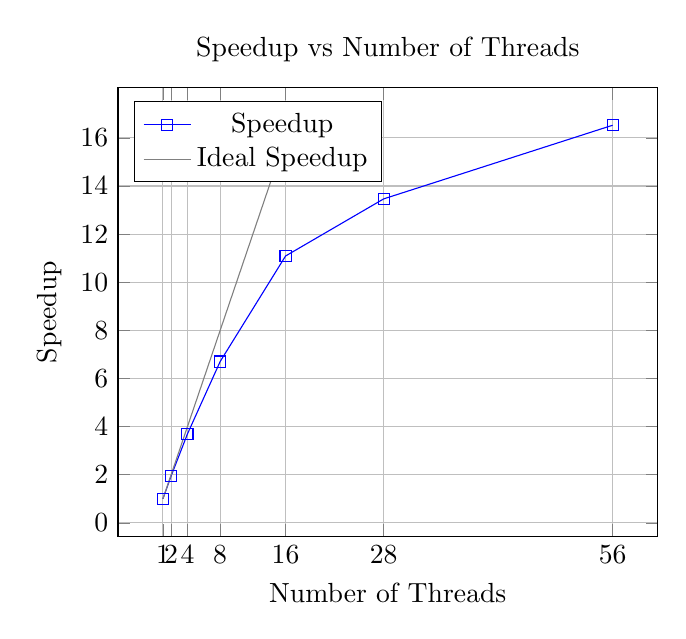
\begin{tikzpicture}
                \begin{axis}[
                    title={Speedup vs Number of Threads},
                    xlabel={Number of Threads},
                    ylabel={Speedup},
                    grid=both,
                    xtick={1, 2, 4, 8, 16, 28, 56},
                    ytick={0, 2, 4, 6, 8, 10, 12, 14, 16},
                    legend pos=north west
                ]
                \addplot[
                    color=blue,
                    mark=square,
                    ]
                    coordinates {
                    (1, 1)
                    (2, 3272 / 1680)
                    (4, 3272 / 885)
                    (8, 3272 / 488)
                    (16, 3272 / 295)
                    (28, 3272 / 243)
                    (56, 3272 / 198)
                    };

                    \addplot[
                    color=gray,
                    ]
                    coordinates {
                    (1, 1)
                    (16, 16)
                    };
                \addlegendentry{Speedup}
                \addlegendentry{Ideal Speedup}
                \end{axis}
                \end{tikzpicture}
            }
        \end{column}
            \begin{column}{0.5\textwidth}
                \begin{figure}
                    \centering
                    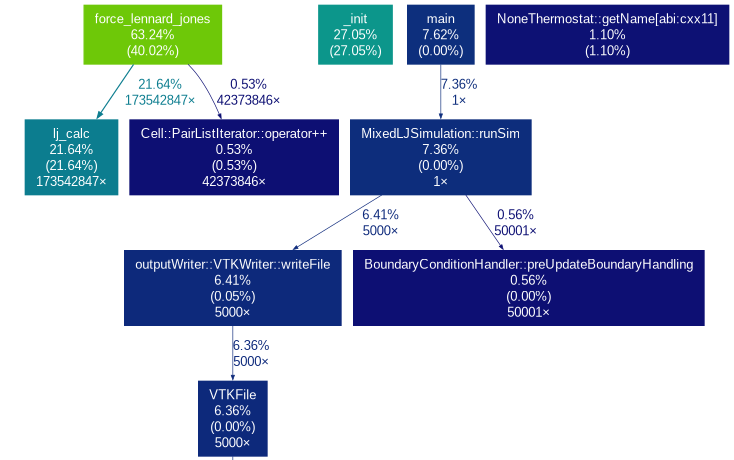
\includegraphics[width=\columnwidth]{../../res/optimized.png}
                    \caption{Visualization of runtime distributions.}
                    \label{fig:runtime}
                \end{figure}
            \end{column}
    \end{columns}
\end{frame}